\hypertarget{covid-introduction-covid-19-and-episim}{%
\section{Introduction: COVID-19 and EpiSim}\label{introduction-covid-19-and-episim}}

In February 2020, the team at VSP began work on an extension to MATSim which became known as ``EpiSim''. The EpiSim model is a novel hybrid of the agent-based microsimulation model MATSim and epidemiological disease progression models.

In the frenetic early days of the COVID-19 pandemic in Europe, new versions of the combined model were being released, tested, and run multiple times per week. This produced massive amounts of data from hundreds of model simulations -- often daily.

By March 2020 the team began publishing initial papers describing the EpiSim model\footnote{These early working papers are all available at \url{https://vsp.berlin/publications/vspwp-episim/}}, and the model itself was very rapidly accruing new features and capabilities.

It quickly became apparent that the team needed a way to compare all of these runs in a visual manner, and also to be able to convey salient results to decisionmakers and the public. A web-based solution was an obvious choice for both use cases, but the many problems encountered in modifying and enhancing MatHub made us unsure that a heavyweight client/server solution would be able to keep up with the team's rapidly changing needs.

The main and urgent challenge to be solved was, how to leverage the investments already made in web-based visualization technologies while increasing velocity and the ability to support the EpiSim team? This chapter describes the novel approach of jettisoning almost all of the back-end server capabilities: instead, a so-called \gls{SPA} was rapidly built that was a completely self-contained website with no back-end server processing at all. All of the website code and all of the data files would be served ``statically'' from a simple web server.

Eventually the size of the site expanded and the data storage for model results migrated to a dedicated file server, but otherwise the overall architecture remained constant and the site remains in operation today.

This approach proved successful in meeting the team's needs, and is described fully in this chapter.

The COVID-Sim website is available at \url{https://covid-sim.info}

% -------------------------------------------------------
\hypertarget{covid-throw-away-the-servers}{%
\section{Throwing away the servers: the EpiSim single page application}\label{covid-throw-away-the-servers}}

As described previously in Chapter \ref{ch:server-experiments}, web sites always consist of the content which is loaded into a browser, known as the ``client'', and the back-end servers which the client connects to in order to receive that content. In the simplest case, a user points to a URL, and the browser loads the HTML index file at that location along with any other static files referenced in the HTML. This is known as a ``static'' website, as the web server does not need to do any dynamic processing to serve the request; it simply delivers the requested files over the network.

Of course, much more complex arrangements are also possible. The web server can run code or scripts which generate part of the page dynamically, can call APIs which pull data from other servers or databases, and so on. These are known as ``dynamic'' sites, and for example the MatHub project described in Chapter \ref{ch:mathub} uses this arrangement.

The MatHub experience highlighted some disillusionment with the state of client/server operations for a data-heavy site such as this. And for EpiSim the problems were expected to be magnified even further: with continual (sometimes daily) modifications to the configuration of the EpiSim model, maintaining parity between the front-end code and back-end databases seemed like an \emph{utter impossibility}, and was certainly not something that could be done at the velocity that the EpiSim analysis team needed.

But if the back-end server database and configuration was slowing development down, would it be possible to just... \emph{eliminate that entire class of problems by eliminating the back-end servers?}

As early as 2003, pioneers in web development including luminary Douglas Crockford, who invented the ``JSON'' data transfer format, were discovering that JavaScript-based websites could actually be far more interactive than the current state of affairs, without any plugins such as Flash or Java virtual machines\footnote{A useful interview with Mr. Crockford about that era is available at the podcast \url{https://corecursive.com/json-vs-xml-douglas-crockford}}. When Google released Gmail in 2004, the floodgates opened for a new class of web-based product called a \gls{SPA}. These types of sites are now everywhere. An SPA site runs JavaScript locally in the browser to transform the page contents that arrive from the web server. This often makes a page feel more interactive or more like a native desktop app. Some of the most popular websites in existence, such as Gmail, Twitter and Facebook, employ this architecture. And by 2015, entire books on the technique were common (see \cite{Scott2015spa}).

Contrast this with the more traditional client/server architecture that frameworks such as PHP or Ruby on Rails employ: a network request from a browser client results in code running on the server which then builds and returns an HTML page to the client. Crucially, the SPA approach allows for user interactions to modify the content of a page without requiring a round-trip data request to a support server. Once the page is loaded, the SPA is ready. Further API calls are allowed, of course, which means data can be queried from external sources as needed. But the essential JavaScript code which drives the website functionality is delivered to the browser first and runs there.

\hypertarget{covid-single-page-application}{%
\subsection{The COVID-Sim single page application}\label{covid-single-page-application}}

This single-page application approach seems ideal for the needs of this project. All of the server functionality is eliminated, except for simple file storage. There is no need for backend server databases, which removes any synchronization problems with the front end code. And the client JavaScript code simply downloads the model output files from the webserver as easily as it loads an image file or any other resource. There is no longer any need to modifying server code every time a new version of the EpiSim model adds new parameters.

The JavaScript libraries described in Chapter \ref{ch:server-experiments} such as Vue and Plotly allow the client-side code to behave similarly to a rich desktop application -- the code connects user interactions (button clicks, mouseovers, etc.) with logic actions such as loading scenario files and drawing the relevant charts.

Thus was created the first simple single page application for EpiSim which loads a basic HTML template, a zipfile with all summary model run outputs, and the view logic to display interactive line charts of pandemic progression over time, along with a set of slider bars that select pandemic intervention approaches. A screenshot of the initial version of the website application, now called COVID-Sim.info, is shown in Figure \ref{fig:covid-v1}.

\begin{figure}
  \centering
	\begin{minipage}{0.8\textwidth}
    \includegraphics[width=\textwidth]{chapters/21-covid-sim/images/covid-v1.png}
  \caption{First version of COVID-Sim.info interactive simulation result explorer.}
  \label{fig:covid-v1}
	\end{minipage}
\end{figure}

The initial interventions being considered were: \emph{Close Public Transit}, \emph{Close Workplaces}, \emph{End Social Activities}, and \emph{End All Other Activities}. Each of these interventions could be user-selected at a given timepoint, measured from ``Never'' to 10, 20, or 30 days after the start of the pandemic. Notably, these were the early days before many other measures such as mask mandates, school closures, or eliminating air travel were available -- and vaccination programs were still very far off in the future.

The site was operational internally in a matter of days, and made public on March 30, 2020\footnote{The COVID-Sim website is online at \url{https://covid-sim.info} and the initial versions can be viewed from the top navigation bar under the heading ``Other Versions''}.

The first versions of the site were produced rapidly and were quite crude, for example with no overall site navigation and almost nothing in terms of exposition. As the project (and pandemic) continued, more model versions were developed and each previous version was archived (and accessible) for reference and comparison.

\hypertarget{covid-cataloging-model-input-parameters-and-the-resulting-model-outputs}{%
\section{Cataloging model input parameters and the resulting model outputs}\label{cataloging-model-input-parameters-and-the-resulting-model-outputs}}

As EpiSim gained complexity, so did the model output website. The number of simulations ballooned to hundreds or thousands of runs per week, and new versions of the model itself were developed both to improve results and to answer decisionmaker questions about the latest turns of the pandemic -- whether that be mask mandates, school closures, vaccination strategies, boosters, etc.

To keep up with this churn, the data visualization strategy was also continually modified. In particular, a new way of mapping the multitude of inputs to the run identification numbers (``Run IDs'') was developed, as the initially small handful of four slider bars was replaced by groups of buttons aligned into logical sets; every combination of which would reference one specific model run.

The combinatorial nature of these options made it imperative to adopt an automated process for identifying model outputs, as well as a way to navigate between different versions of the model itself.

\hypertarget{covid-describing-simulations-using-yaml}{%
\section{Describing simulations using YAML}\label{covid-describing-simulations-using-yaml}}

The solution to this proliferation of simulation options and scenarios is comprised of two pieces of data for each batch of simulations:

\begin{itemize}
  \tightlist
  \item
  First, a simple lookup table that establishes the connection between the run-identification numbers and the specific input parameter values for every parameter in the model. For example, a batch of runs simulating four different mask strategies and two school closure strategies has 4x2 so eight combinations of parameters; therefore the lookup table has exactly eight rows. Each row specifies the Run ID for the value of the two hypothetical parameter values in that run. In reality, there are always far more than eight combinations; often 768 or 1,024 different permutations of a dozen parameters are tested, all batched together in a nightly run on the University high-performance compute cluster. This lookup table is stored as a simple text file in CSV format.
  \item
  Second, for the display of available options to users of the EpiSim dashboard, a human-readable and user-interface friendly mapping between the Run ID, option groups, variable names, and values is also needed. This second input file went through many iterations before finding a satisfactory approach.
\end{itemize}

Most variables in EpiSim are either general in nature, affecting the entire simulation; or time-based, occurring on specific dates or ``N days after'' the start of the simulation. This time-based aspect of EpiSim leads to a natural grouping of parameters, making the many user interface options more digestible for non-experts in EpiSim.

The EpiSim parameters themselves are usually numeric or categorical; each variable can have multiple values that also have a human-interpretable meaning. For example the percentage of people wearing masks on transit; or the types of masks being worn (\emph{N95, surgical, none}).

Capturing all of this information in a definable, repeatable format for use in the user interface required something more structured than the simple lookup table above.

For this, a well-known and common configuration file format known as \gls{YAML} is used.\footnote{The YAML standard is defined at \url{https://yaml.org/}}. YAML excels at describing sets of \emph{key:value} relationships and allows lists and grouping of keys underneath other keys. It is human-readable and computer-parseable; these traits lead to YAML being a popular format for specifying configuration information in myriad of software systems.

For a batch of EpiSim runs, the operator of EpiSim produces the lookup table with the specific model parameters and a YAML file containing the metadata that describes in human terms how the variables will be presented to the user in the dashboard.

An example YAML file is listed in Figure \ref{fig:covid-yaml}: this is abbreviated for clarity. More complex model runs have more sections and more variables defined.

\begin{figure}
  \centering
	\begin{minipage}{0.9\textwidth}
    \centering
    \includegraphics[width=0.7\textwidth]{chapters/21-covid-sim/images/covid-yaml.png}
  \caption{Example YAML text-based configuration for a set of COVID-Sim simulation runs. Note groups of settings which activate on specific days in the simulation.}
  \label{fig:covid-yaml}
	\end{minipage}
\end{figure}

\begin{figure}
  \centering
	\begin{minipage}{0.9\textwidth}
    \includegraphics[width=\textwidth]{chapters/21-covid-sim/images/covid-buttons.png}
  \caption{Example simulation output showing left-panel selection buttons, based on YAML configuration.}
  \label{fig:covid-buttons}
	\end{minipage}
\end{figure}


\hypertarget{covid-retrieving-model-results}{%
\section{Retrieving model results}\label{retrieving-model-results}}

The final piece of the puzzle is the storage and retrieval of the actual model results.

A batch of simulation runs produces summary outputs for every combination of model parameters. Those outputs are identified by the Run ID defined above, and they are compressed into a single .ZIP format file archive. The contents of the .ZIP file vary based on what version of the model was run: early versions only included daily disease progression statistics (i.e., the number of simulated people who are susceptiple, infected, contagious, sick, and so on). Later versions added many additional outputs such as disease import from other areas, vaccination rates, levels of multiple virus strains in the wild, and more.

Thus a full batch output, ready for display in the COVID-Sim website,
includes:

\begin{itemize}
\item
  \textbf{info.txt}: the lookup table of simulation Run IDs along with the specific
  values for every model parameter used; one row per simulation.
\item
  \textbf{metadata.yaml}: the collection of descriptive names for each model parameter,
  usually grouped into logical or time-based categories
\item
  \textbf{summary.zip}: a compressed folder containing the CSV-formatted outputs for one
  specific run. This file is usually named according to the Run ID number for that simulation.
\end{itemize}

These files are stored on the departmental file server in hierarchical folders, organized by run date, city, and many other categories. Once these files are uploaded to the file server, they can be accessed via HTTP by the COVID-Sim website, and, in fact, by anyone on the Internet as the simulation output files are all completely public.

The COVID-Sim website maps the requested URL directly to the file structure on disk: so for example, \emph{http://covid-sim.info/2021/11/05/example-run} displays results stored in the \texttt{2021/11/05/example-run} folder on the file server. Thus the website has complete access to all of the metadata and summary .ZIP files, and can download any user selection as needed, precisely when requested by the user.

\hypertarget{covid-architecture}{%
\section{Architecture}\label{architecture}}

With all these pieces in place, the novel and unique overall architecture of the EpiSim data visualization portal emerges:

\begin{itemize}
\item
  An ``SPA'' single page application, based on JavaScript, the Vue interaction library, and various graphic and charting libraries. This application is hosted on a simple, static website hosting provider,
\item
  Hierarchical file storage on a university departmental file server,
  with data for all published runs accessible via HTTP. Each run is
  stored in its own folder, and contains:

  \begin{itemize}
  \item
    Automatically-generated configuration files, produced when the
    EpiSim simulation runs are set up. These describe the specific
    combinations of input parameters that are to be run.
  \item
    A lookup table which maps each combination of input parameters to a
    specific output dataset ID
  \item
    Zipped output files containing the summary data for each simulation
    run, identifiable by the ID codes specified in the above lookup table.
  \end{itemize}
\item
  A set of interactive charts, animations, and descriptive pages which depict the
  contents of the selected simulation outputs. These views update immediately when
  the user selects a new simulation from the available options.
\end{itemize}

The types and number of charts and visualizations have grown considerably since the beginning of the project in March 2020. A considerable effort has been made to be nimble and add new visualizations as soon as the analyst team identifies a new need, or produces a new type of simulation output. These charts now run the gamut of disease progression, hospitalization rates, R-value statistics, age-related effects, vaccination rates, activity levels by activity type, and much more.

\hypertarget{covid-animations-of-infection-progression-in-berlin}{%
\section{Animations of infection progression in Berlin}\label{animations-of-infection-progression-in-berlin}}

A secondary goal of the site is to be an external-facing portal for educating decisionmakers, the media, and the public. Internal analysts much appreciated the ability to compare results of model runs by flipping switches and sliders and seeing how the model output graphs reacted. But as the team took the results to non-experts, it was clear that something else was also needed: a visual representation of how the model actually worked.

The agent-based model is based on the daily activities and movements of every population member, interacting with each other, spreading the infection when contagious, and then having the disease progress. This is well-suited to an \emph{animation of the agents moving through time and space}. Such an animation was included between versions 2 and 4 of the EpiSim model itself. These animations depict the ``do nothing'' scenario for Berlin: in other words, how the COVID-19 pandemic would proceed through Berlin and the surrounding areas if no measures were ever taken at all to combat it.

The infection status of each agent is represented by color: susceptible, infected, contagious, sick, seriously sick (hospitalized), critical (intensive care), and recovered agents each have a different color. Their motions can be seen over the course of a day and over the 90-day course of the pandemic simulation.

Any specific day in the simulation can be chosen from a panel to see the infection status of the population on that day. The exponential nature of the pandemic is very clearly illustrated in this manner.

A second animation was added later that removed the daily back-and-forth motion of agents on individual trips, and simply showed the status of agents at their home locations, over the course of the 90-day simulation.

The animation technology used for these visualizations helped to significantly inform later projects described in Chapters \ref{ch:avov}, \ref{ch:pave}, and \ref{ch:simwrapper}.

Figure \ref{fig:covid-animation} shows some snapshots in time of the animation progression, for a 90-day pandemic simulation for Berlin.

\begin{figure}
  \centering
	\begin{minipage}{\textwidth}
    \centering
    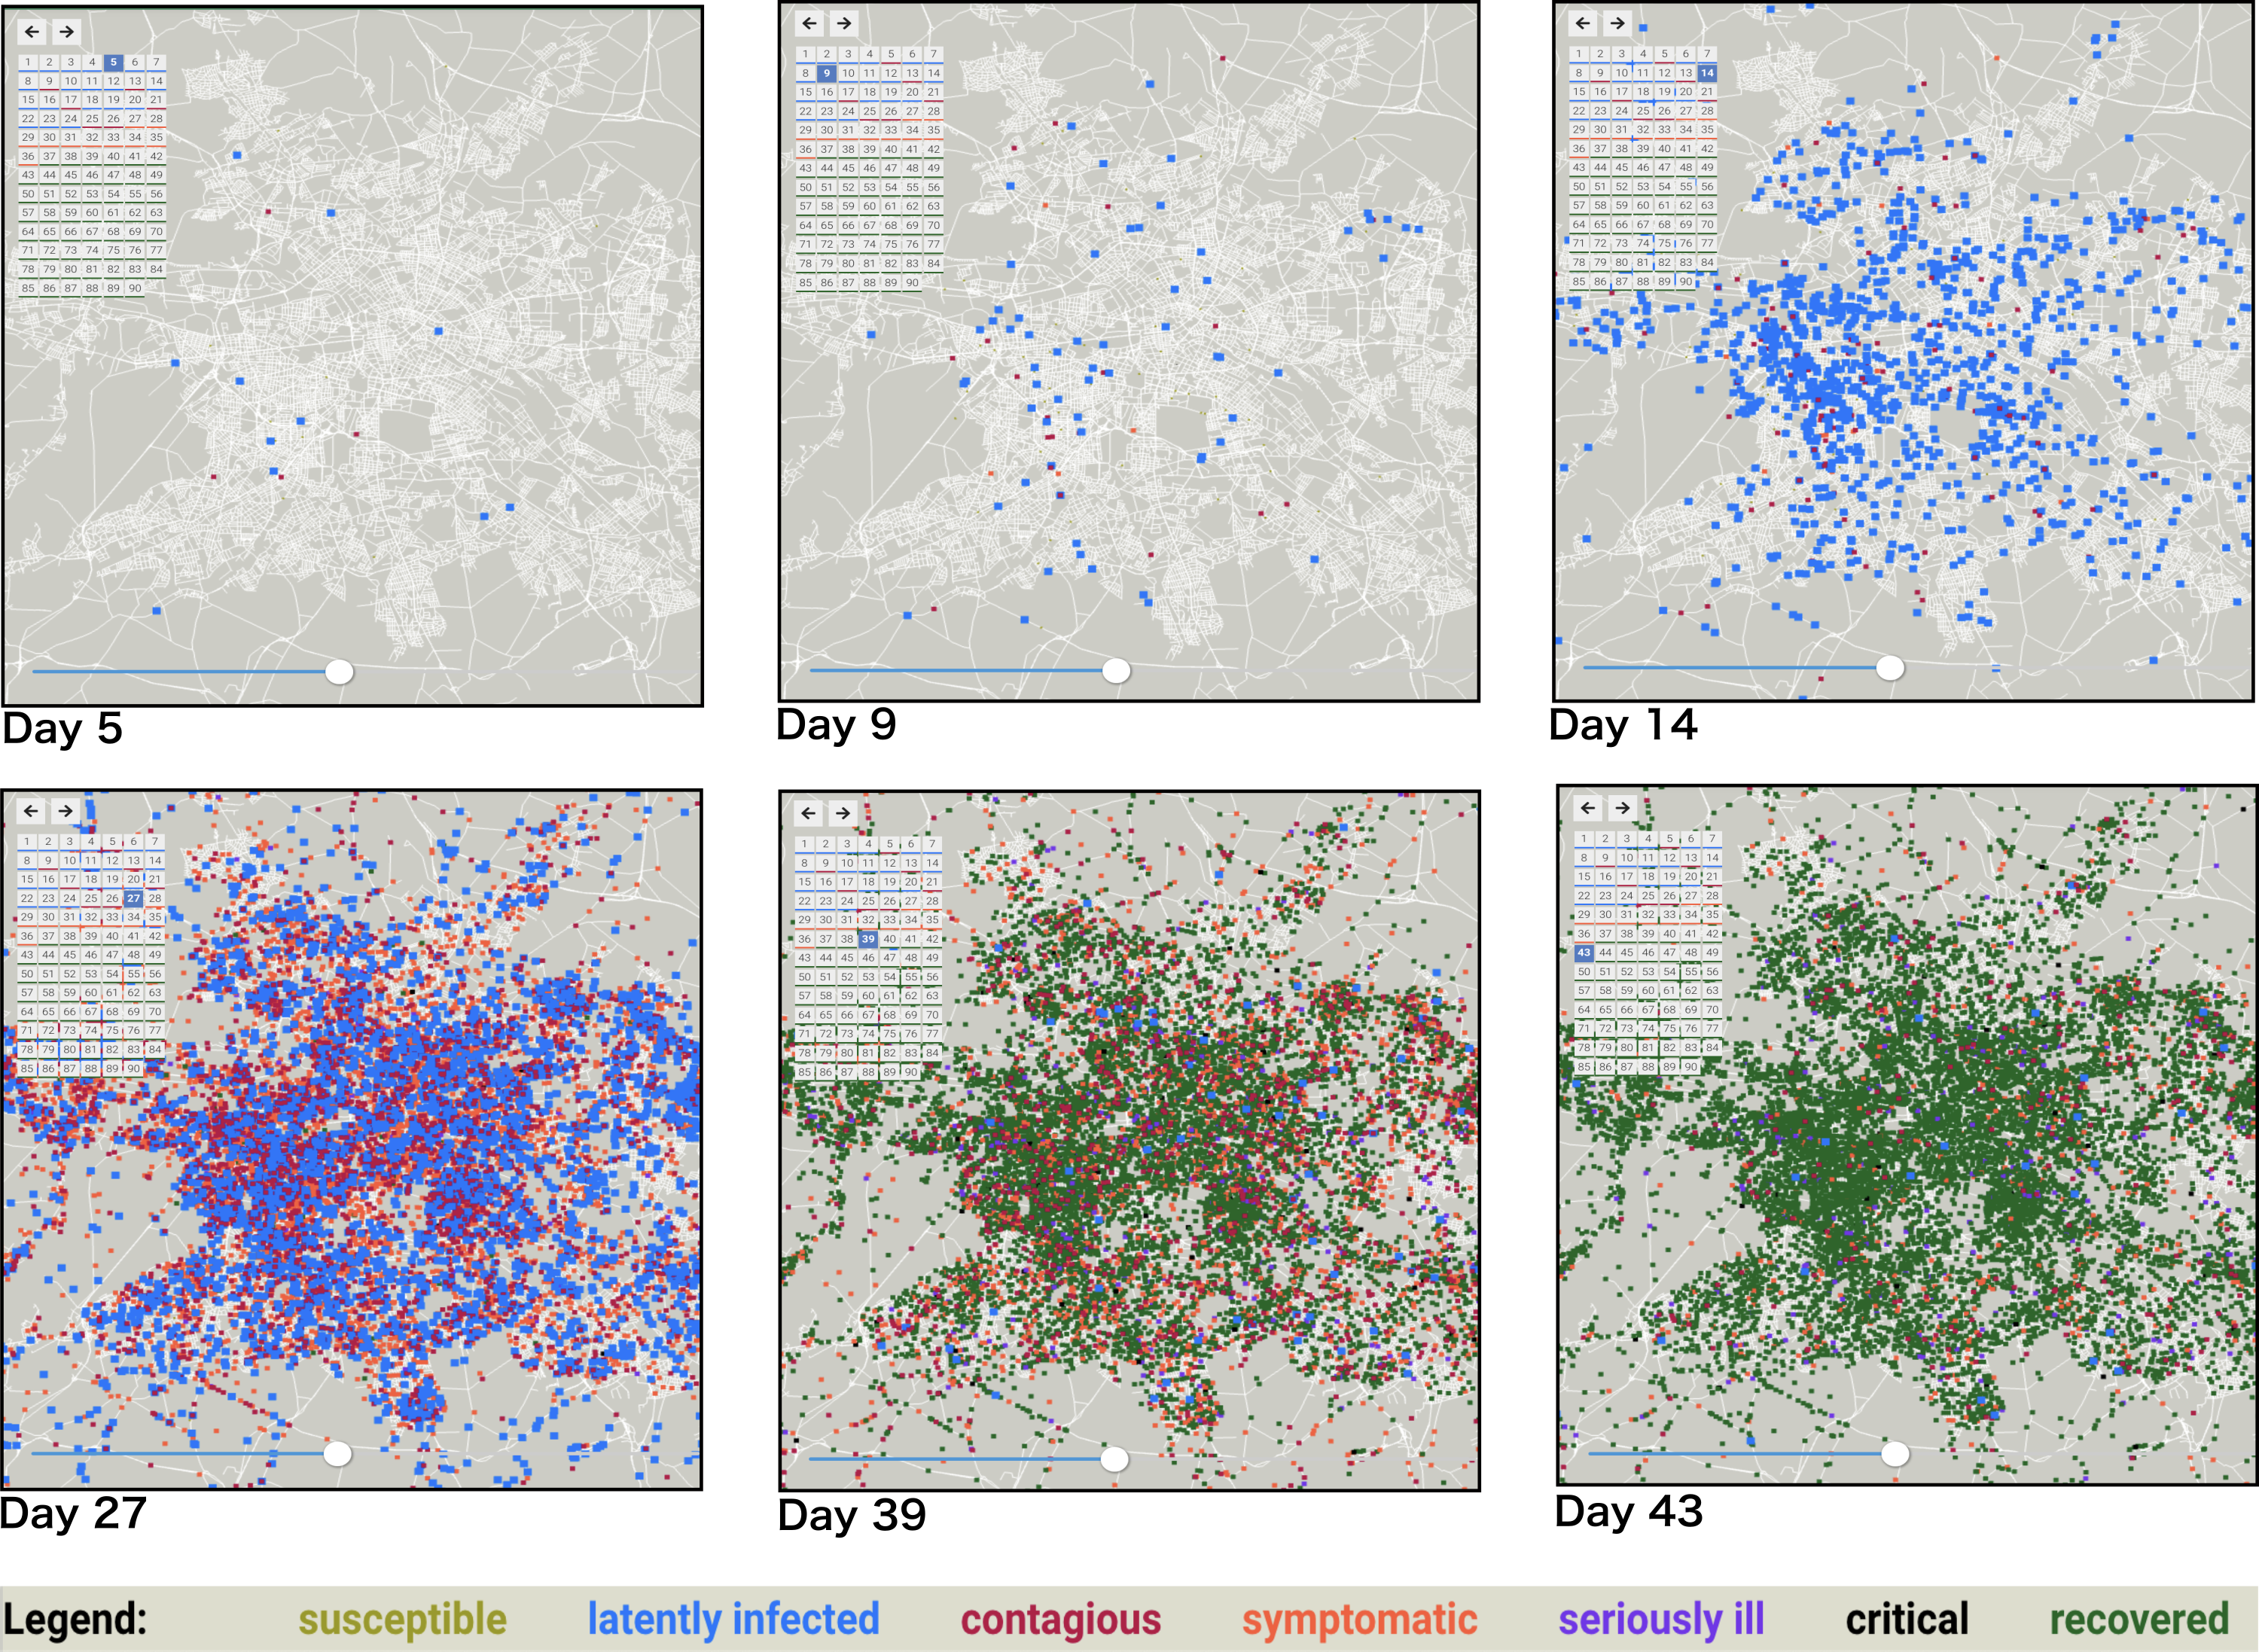
\includegraphics[width=\textwidth]{chapters/21-covid-sim/images/covid-animation.png}
  \caption{Sample animation of COVID-19 disease progression in Berlin, for six snapshot days in the 90 day simulation.}
  \label{fig:covid-animation}
	\end{minipage}
\end{figure}

% ==============================================
\hypertarget{covid-discussion}{%
\section{Discussion}\label{covid-discussion}}

At the outset of the EpiSim effort in March 2020, it was unclear how much anyone outside the research group would be interested in this work. The first results and the animations were put together in great haste, a matter of weeks, with the idea that the results might have great public interest.

That major public interest never quite materialized. The project lead, Professor Kai Nagel, made great efforts to get the model published in peer-reviewed scientific journals, made connections with other researchers for collaboration, and also engaged the public, the media, and the political system in Berlin and in Germany throughout 2020 and beyond. The website itself, however, found a much smaller niche: for the most part, its users were the internal analyst staff who needed to compare, understand, and debug the thousands of runs that they were producing. The iterative nature of the development led to a proliferation of detailed charts and graphs which probably was not suitable to a truly outward-facing public website. But the project team found great value in the site, both in the office and when they went to present findings to others.

% ----------------------------------------------
\hypertarget{covid-user-feedback}{%
\subsection{User feedback}\label{user-feedback}}

No user experience surveys were performed while building this analysis portal, as its rapid development precluded any regimented and carefully designed study. Instead, constant weekly feedback from the users of the site was ad-hoc in nature.

In general, the site was considered to be extremely useful, and the automated nature of the process from simulation completion to visible, comparable results online, was lauded many times over.

There were several rounds of design changes in both the automation pipeline and in the website display functionality, mostly completed in the first several months of work. Ultimately the number of modifications grew so great, with commensurate bugs popping up in old versions of runs, that a ``split'' was decreed which froze the older runs onto a ``Viewer Version 1'' copy of the site, while newer runs would receive the latest updates. This alleviated much stress about user testing the hundreds and hundreds of runs on the site after every set of changes.

Feedback on the animations revealed that, while they look nice (according to analyst staff), they did not prove particularly useful after the initial months of the COVID-19 pandemic. Users did say that the animations were helpful in the spring of 2020 to help describe how the model worked.

% ----------------------------------------------
\hypertarget{covid-iteration-and-further-work}{%
\subsection{Iteration and further work}\label{covid-iteration-and-further-work}}

The site continues to receive updates to support new model versions. No new major features are currently planned, and the infrastructure seems to be holding up very well.

Possible future work could include a user interface overhaul to reign in the proliferation of charts and graphs. The ``one long vertical list'' of charts is helpful for aligning timelines on the x-axis, but it is not an excellent user experience. Some detailed design work might reveal that a more standard ``dashboard'' approach might also be valuable.

% ----------------------------------------------
\hypertarget{covid-informing-decisionmaking-with-comparison-dashboards}{%
\section{Conclusion: Informing decisionmaking with comparison dashboards}\label{covid-informing-decisionmaking}}

The ability to rapidly visualize and assess the results of thousands of simulations runs is crucial to the team's ability to support ongoing decisionmaking on this project. Advanced simulations like MATSim, ActivitySim, and EpiSim produce so much data that visualization and assessment are absolutely essential for deep understanding of the outputs.

By all measures, the COVID-Sim simulation portal is a resounding success story. Transport modelers are very rarely so close to the decisionmaking apparatus, helping in a small way to answer urgent questions that tangibly affect society. The fact that the lessons learned in the simple experiments of Chapters \ref{ch:server-experiments} and \ref{ch:mathub} proved so useful so soon, is a breathtaking and satisfying outcome.
